\documentclass[12pt]{article}
\usepackage{natbib}
\usepackage[french]{babel}
\usepackage[T1]{fontenc}
\usepackage{url}
\usepackage[utf8x]{inputenc}
\usepackage{lastpage}
\usepackage{amsmath}
\usepackage{hyperref}
\usepackage{graphicx}
\usepackage{pdflscape}
\graphicspath{{images/}}
\usepackage{pdfpages}
\usepackage{parskip}
\usepackage{fancyhdr}
\usepackage{multicol}
\usepackage{vmargin}
\usepackage{float}
\setmarginsrb{3 cm}{2.5 cm}{3 cm}{2.5 cm}{1 cm}{1.5 cm}{1 cm}{1.5 cm}

\title{ThermiScan}
\author{Lorenzo Bauduccio \\ Tom Ryser \\ Kevin Moreno}
\date{\today}

\makeatletter
\let\thetitle\@title
\let\theauthor\@author
\let\thedate\@date
\makeatother

\pagestyle{fancy}
\fancyhf{}
\rhead{Atelier Technicien 1\&2}
\lhead{Rapport - ThermiScan}
\cfoot{\thepage\ sur \pageref{LastPage}}
\rfoot{\footnotesize \thedate}

%$HeadURL: https://subversion.assembla.com/svn/cfpt-courses/trunk/_inc/inc_lst_csharp.tex $
%$LastChangedDate: 2016-10-12 16:29:50 +0200 (Wed, 12 Oct 2016) $
%$LastChangedRevision: 7006 $
%$LastChangedBy: marechal $

% lstlisting configuration for C#
%-------------------------------------------------------------------------------------
\usepackage{xcolor}
\usepackage{listings}
\usepackage{accsupp}

% color
\definecolor{lightgreen}{rgb}	{0.200, 0.980, 0.200}
\definecolor{darkgreen}{rgb}	{0.000, 0.400, 0.000}
\definecolor{lightgray}{gray}	{0.98}
\definecolor{darkred}{rgb}		{0.545, 0.000, 0.000}

% CSharp colors
\definecolor{class}{rgb}		{0.200, 0.600, 0.600}	% Cyan Visual Studio
\definecolor{keyword}{rgb}		{0.000, 0.000, 1.000}	% blue

% code to avoid line number copy during copy-paste from PDF
\newcommand{\noncopynumber}[1]{%
    \BeginAccSupp{method=escape,ActualText={}}%
    {\scriptsize#1}%
    \EndAccSupp{}%
}

% lstlisting parameters
\lstset {	
  language=[Sharp]C
, captionpos=b
, frame=shadowbox
, rulesepcolor=\color{gray}
% syntaxic coloration
, basicstyle=\footnotesize\ttfamily
, keywordstyle=\color{blue}
, commentstyle=\color{darkgreen}
, stringstyle=\color{darkred}
, backgroundcolor=\color{lightgray}
, identifierstyle=\color{black}
% lines numbering
, numbers=left
, numberstyle=\noncopynumber
, stepnumber=1
, numbersep=5pt
%
, breaklines=true
, tabsize=2
, showstringspaces=false
, lineskip={-1.5pt} % single line spacing
, escapeinside={/*(*@}{@*)*/}
, rangeprefix=//\{\  % slash, slash, curly left brace, space
, rangesuffix=\ \} % space, curly right brace
}

% Csharp : additional keywords
\lstset{
	morekeywords={var,get,set,string,value},
	otherkeywords={\#region,\#endregion,\#define,\#if,\#endif,\#else}, %morekeyword does not support # chararacter then we must use otherkeywords
	emph={[1]Application,
		Char,Color,Console,Convert,
		DialogResult,
		Environment,EventArgs,
		Form,
		Object,String,
		Assert,
		SByte,Int16,Int32,Int64,
		Byte,UInt16,UInt32,UInt64,
		Single,Double,
		Keys,KeyPressEventArgs,
		MessageBox,MessageBoxButtons},
	emphstyle={[1]\color{class}}
}

\lstset{prebreak=\raisebox{0ex}[0ex][0ex]
        {\ensuremath{\hookleftarrow}}}
%\lstset{postbreak=\raisebox{0ex}[0ex][0ex]
%        {\ensuremath{\hookrightarrow\space}}}
\lstset{breaklines=true, breakatwhitespace=true}

% replace sequence of char by another sequence of char
% see http://stackoverflow.com/questions/1116266/listings-in-latex-with-utf-8-or-at-least-german-umlauts
\lstset{literate=%
{ä}{{\"a}}1
{â}{{\^a}}1
{à}{{\`a}}1
{Ä}{{\"A}}1
{Â}{{\^A}}1
{À}{{\`A}}1
{ë}{{\"e}}1
{ê}{{\^e}}1
{é}{{\'e}}1
{è}{{\`e}}1
{Ë}{{\"E}}1
{Ê}{{\^E}}1
{É}{{\'E}}1
{È}{{\`E}}1
{ï}{{\"i}}1
{î}{{\^i}}1
{Ï}{{\"I}}1
{Î}{{\^I}}1
{ö}{{\"o}}1
{ô}{{\^o}}1
{Ö}{{\"O}}1
{Ô}{{\^O}}1
{ü}{{\"u}}1
{û}{{\^u}}1
{ù}{{\`u}}1
{Ü}{{\"U}}1
{Û}{{\^U}}1
{Ù}{{\`U}}1
{ç}{{\c c}}1
{Ç}{{\c C}}1
{°}{{\textsuperscript{o}}}1
% suppress BOM (Byte Order Mark) characters at the beginning of Visual Studio source
% see http://tex.stackexchange.com/questions/5935/how-to-suppress-bom-effect-in-the-output
{ï}{}0
{»}{}0
{¿}{}0
}


\begin{document}

%%%%%%%%%%%%%%%%%%%%%%%%%%%%%%%%%%%%%%%%%%%%%%%%%%%%%%%%%%%%%%%%%%%%%%%%%%%%%%%%%%%%%%%%%

\begin{titlepage}
	\centering
    
\includegraphics[scale = 1]{logo-cfpt-site.png}\\[1.5 cm]
    \textsc{\LARGE CFPT Informatique}\\[2.0 cm]
	\textsc{\Large Atelier Techniciens 1\&2 - Rapport}\\[0.5 cm]
	\rule{\linewidth}{0.2 mm} \\[0.4 cm]
	{ \huge \bfseries \thetitle}\\
	\rule{\linewidth}{0.2 mm} \\[1.5 cm]
	
	\begin{minipage}{0.4\textwidth}
		\begin{flushleft} \large
			\emph{Étudiants:}\\
			\theauthor
			\end{flushleft}
			\end{minipage}~
			\begin{minipage}{0.4\textwidth}
			\begin{flushright} \large
			\emph{Enseignant:} \\
			Francisco Garcia
		\end{flushright}
	\end{minipage}\\[2 cm]
	
	{\large \thedate}\\[0.5 cm]
 
	\vfill
	
\end{titlepage}

%%%%%%%%%%%%%%%%%%%%%%%%%%%%%%%%%%%%%%%%%%%%%%%%%%%%%%%%%%%%%%%%%%%%%%%%%%%%%%%%%%%%%%%%%

\setcounter{page}{2}
\tableofcontents
\pagebreak

%%%%%%%%%%%%%%%%%%%%%%%%%%%%%%%%%%%%%%%%%%%%%%%%%%%%%%%%%%%%%%%%%%%%%%%%%%%%%%%%%%%%%%%%%

\section{Cahier des charges}
\subsection{Description du projet}
Nous devons réaliser une application en Web qui doit nous permettre d’afficher une vidéo venant du smartphone CAT S60, qui possède une caméra thermique. L’application Web doit permettre de gérer plusieurs vidéos venant de plusieurs caméras, et permettre d’afficher une courbe de température.
\subsection{Travail à réaliser}
\begin{itemize}
    \item Réaliser une application en Web qui s'approche un maximum d'un point de vue fonctionnel de l'application FLIR Tools Mobile.
    \begin{itemize}
        \item Affichage d’un graphique montrant la température maximal, minimal et la moyenne.
        \item Affichage de la vidéo.
        \item Gestion de plusieurs vidéos venant d’une seule caméra. 
    \end{itemize}
\end{itemize}
\subsection{Outils utilisés}
\begin{itemize}
     \item Visual Studio Code
     \item EasyPHP V 14.1
     \item MySQL
     \item Python 3
     \item Balsamiq Mockups 3
\end{itemize}

\subsection{Comment avons-nous procédé ?}
\begin{itemize}
     \item Réalisation d’une maquette du front-end
     \item Création d’un exécutable à partir d’un programme python
     \item Création d’une base de données pour les utilisateurs, les caméras et les vidéos
     \item Réalisation du front-end avec easyPHP
     \item Ajout d’un script JS permettant d’afficher un graphique
     \item Mise au propre du code
\end{itemize}

\clearpage

\subsubsection{Installation de Tesseract}
    \begin{enumerate}
        \item Exécuter dans le cmd \textit{pip install pytesseract}
         \item Télécharger Tesseract OCR sur \url{https://digi.bib.uni-mannheim.de/tesseract/tesseract-ocr-w64-setup-v5.0.0-alpha.20200223.exe} et faire l'installation par défaut.
        \item Déplacer le dossier contenu dans le .zip sous \path{C:\Program Files}.
        \item Dans la barre de recherche Windows, taper \textit{"Modifier les variables d'environnement système"}.
        \item Cliquer sur le bouton \textit{"Variable d'environnement"} en bas de la page.
        \item Cliquer sur \textit{"Nouvelle..."} pour les variables d'administrateur.
        \item Nom de la variable : \texttt{TESSDATA\_PREFIX}.
        \item{Cliquer sur \textit{"Parcourir le répertoire"} et sélectionner Tessdata sous \path{C:\Program Files\tesseract-OCR\tessdata}}
    \end{enumerate}

\subsubsection{Installation de Python 3.8}
    \begin{enumerate}
        \item Aller sur le site de python : \url{https://www.python.org/downloads/release/python-382/}
        \item Prendre \textit{Windows x86 executable installer}.
        \item Au début de l'installation, sélectionner \textit{Add Python 3.8 to PATH}.
        \item À la fin de l'installation, cliquer sur \textit{Disable Path Length limit}.
        \item Après l'installation de Tesseract, Ouvrir le cmd et aller dans le dossier \texttt{pythonApp} du projet et exécuter dans le cmd \textit{pip install -r requirements.txt}
    \end{enumerate}
\subsection{Github}
    \url{https://github.com/Ryser-tom/ThermiScan.git}
\clearpage

\section{Réalisations}
\subsection{base de données}
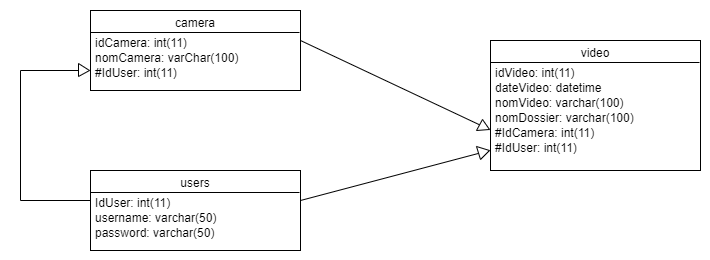
\includegraphics[scale = 0.5]{diagram.png}\\
\begin{itemize}
        \item Camera : Stock le nom des differentes camera des utilisateurs. 
        \item Video : Stock les information des video comme la date d'ajout et la camera associer a la video.
        \item Users : Stock le nom d'utilisateur et les mot de passe des diferents utilisateurs.
    \end{itemize}

\subsection{Description du code}
\begin{table}[H]
\caption{function.php}
\resizebox{\textwidth}{!}{\begin{tabular}{|l|l|}
\hline
Nom & Paramètres \\ \hline
GetListOfvideoCameraVue(\$idCamera) & retourne sous forme de lien toutes les videos \\ 
                                    & en lien avec une camera ou toutes les videos \\ \hline
GetListOfCameraVue()                & retourne la liste des cameras sous forme de lien \\ \hline
GetListOfCameraUserVue()            & retourne la liste des cameras sous forme d'option \\
                                    & pour formulaire \\ \hline
GetInfosVideo(\$videoId)            & retourne les informations d'une video \\ \hline
GetFirstCameraUser()                & retourne une camera de l'utilisateur connecter \\ \hline
\end{tabular}}
\end{table}

\begin{table}[H]
\caption{user.php}
\resizebox{\textwidth}{!}{\begin{tabular}{|l|l|}
\hline
Nom & Paramètres \\ \hline
\_\_construct(\$username, \$idUser) & Constructeur de la classe \\ \hline
GetUsername()                       & retourne le nom d'utilisateur de l'utilisateur \\ \hline
GetIdUser()                         & retourne l'id de l'utilisateur \\ \hline
GetListOfCameraUser()               & retourne la liste des cameras de l'utilisateur \\
GetListOfVideo()                    & retourne toutes les videos d'un utilisateur \\ \hline
GetListOfVideoByCamera(\$idCamera)  & retourne la liste de video liée a une camera \\ \hline
\end{tabular}}
\end{table}

\begin{table}[H]
\caption{pdo.php}
\resizebox{\textwidth}{!}{\begin{tabular}{|l|l|}
\hline
Nom & Paramètres \\ \hline
\_\_construct(\$host, \$dbname, \$user, \$password) & Constructeur de la classe \\ \hline
CreateConnexion()                           & Crée une connexion à la BDD \\ \hline
Select(\$select, \$from, \$where, \$order)  & Permet d’executer un select de façon simple \\ \hline
Delete(\$from, \$where)                     & Permet d’executer un delete de façon simple \\ \hline
Update(\$from, \$set, \$where)              & Permet d’executer un update de façon simple \\ \hline
Execute(\$requete)                          & Execute la requete SQL passer en paramètre \\ \hline
SelectFull(\$select)                        & Retourne le resultat de la requete passée en paramètre \\ \hline
\end{tabular}}
\end{table}

le fichier \texttt{background.py} détecte si une modification a eu lieu dans le dossier \textit{toDo}, et envoie le chemin du fichier \textit{video.mp4} à \texttt{extract.py}.
\subsubsection{background.py}	
\lstset{language=Python}
\begin{lstlisting}
import extract  # For the image script

import logging  # To create easy log file
import time  # For the time.sleep
import threading # For 
import os
import shutil #To move the folder
import pytesseract as pyt

# For the file detection, It doesn't work on 64-bit
from watchdog.observers import Observer
from watchdog.events import FileSystemEventHandler

# configuration for the logging function
logging.basicConfig(filename='app.log',
                    filemode='a',# filemode='a' is for append
                    format='%(asctime)s - %(message)s',
                    datefmt='%d-%b-%y %H:%M:%S')

#class that wait for an event, when it get's an event it call the Handler class and give him the event
class Watcher:
    DIRECTORY_TO_WATCH = "../web/file/toDo"
    
    def __init__(self):
        self.observer = Observer()
        pass

    def run(self):
        event_handler = Handler()
        self.observer.schedule(event_handler,
                               self.DIRECTORY_TO_WATCH,
                               recursive=True)
        self.observer.start()
        try:
            while True:
                time.sleep(5)
        except:
            self.observer.stop()
            print("Error")

#called if an event occured
class Handler(FileSystemEventHandler):
    @staticmethod
    def on_any_event(event):

        # global is used to tell that we will modifiy the global variable
        global folderName

        # event_type can be : created, modified, deleted
        # is_directory is used to tel if the event concern a folder or not by a boolean
        if event.event_type == 'created' and event.is_directory == False:

            # example of event.src_path '../web/file/toDo\ 
            # 8675ab54b50cc355a5665dd33827806c14fbe71b\video.mp4'
            path = event.src_path.split('/')
            print(event.src_path)
            path2 = path[3].split('\\')

            # example of source '../web/file/toDo/
            # 8675ab54b50cc355a5665dd33827806c14fbe71b'
            source = path[0] + "/" + path[1] + "/" + path[2] + "/" + path2[0] + "/" + path2[1]

            # example of destination '../web/file/done'
            #destination is used when moving the folder at the end.
            destination = path[0] + "/" + path[1] + "/" + path[2] + "/" + "done"
            
            # test if the file is the video.mp4, and the folder is diffrent than the last one (to prevent the script from running twice on the same video)
            if path2[-1] == 'video.mp4' and folderName != path2[-2]:
                folderName = path2[-2]
                print('event type: ' + event.event_type + ' and is a directory: ' + str(event.is_directory) + ' name is: ' + path2[-1] + ' source is :' + folderName)

                # prepare the function that will be called as a thread, and then start the thread
                thread = threading.Thread(target=extract.extractFrames(event.src_path, source))
                thread.start()

                # wait here for the end of the thread before continuing
                thread.join()
                logging.warning('The file at %s has been added' % event.src_path)


                # Try to move the folder now that the script is almost finished.
                try:
                    shutil.move(source, destination)
                    print('The folder as been moved.')
                except:
                    pass
                    print("An exception occurred, could not move the folder")
            
            


if __name__ == '__main__':
    folderName = ''
    scriptDirectory = os.path.dirname(os.path.realpath(__file__))
    print('start: background script for Thermiscan project!')
    w = Watcher()
    w.run()
\end{lstlisting}

le fichier \texttt{extract.py} lit la vidéo dans le chemin spécifié par \texttt{background.py}, et il en extrait les images pour les envoyer à \texttt{image.py}.
\subsubsection{extract.py}
\begin{lstlisting}
import image

# Importing all necessary libraries
import cv2 # For the text recognition
import os 
import csv # To write the csv

# Read the video from specified path
path = "..//video//vidTest.mp4"
def extractFrames(path, folderSource):
    print('start extract.py')
    cam = cv2.VideoCapture(path)
    try:
        # creating a folder named data
        if not os.path.exists('/data'):
            os.makedirs('/data')
            
    # if not created then raise error
    except OSError:
        print('Error: Creating directory of data')

    # frame counter
    currentframe = 0
    print(cam)

    while (True):

        # reading from frame
        ret, frame = cam.read()

        if ret:
            # if video is still left continue creating images
            name = './data/frame' + str(currentframe) + '.jpg'

            # writing the extracted images to be processed in image.py
            cv2.imwrite(name, frame)
            image.read_break_image(currentframe, frame, folderSource)
            currentframe += 1
        else:
            break

    # Release all space and windows once done
    print('extract done')
    cam.release()
    cv2.destroyAllWindows()
\end{lstlisting}

le fichier \texttt{image.py} est appelé pour traiter une image et enregistrer ses valeurs dans un CSV.
\subsubsection{image.py}
\begin{lstlisting}
import csv
import re
import os
import sys
import numpy as np
from PIL import Image
import cv2
import pytesseract as pyt
#uncomment the next line to execute on Windows
pyt.pytesseract.tesseract_cmd = r'C:\\Program Files\\Tesseract-OCR\\Tesseract.exe'
regex = r"\d+\,\d+"

def read_break_image(frame, image, folderSource):
    
    # Set minimum and max HSV values to display
    lower = np.array([0, 0, 250])#0,0,0
    upper = np.array([179, 70, 255])#179,70,255

    # Create HSV Image and threshold into a range.
    hsv = cv2.cvtColor(image, cv2.COLOR_BGR2HSV)
    mask = cv2.inRange(hsv, lower, upper)
    output = cv2.bitwise_and(image,image, mask= mask)
    img_to_read = cv2.bitwise_not(output)
    img_to_read = img_to_read[0:110, 10:240]

    cv2.imwrite('out.png', img_to_read)
    text = pyt.image_to_string(img_to_read)
    write_csv(text, frame, folderSource)


def write_csv(row, frame, folderSource):
    with open(folderSource + '/value.csv', 'a', newline='') as outfile:
        writer = csv.writer(outfile,  delimiter=';',
                            quotechar=' ', quoting = csv.QUOTE_NONNUMERIC)
        #data_writer.writerow(['Min', 'Moy', 'Max'])
        
        matches = re.findall("\d+\,\d+", row)
        if len(matches) == 3:
            writer.writerow([frame, matches[2], matches[0], matches[1]])
            #print(frame, 'OK')
        else:
            print('dead')
            print(matches)

if __name__ == '__main__':
    #print('image file.started.')
    read_break_image("capture.png")
    #print('End of image.py script')

\end{lstlisting}

\section{Conclusion}
\subsection{Bilan}
Dans l’ensemble, nous sommes plutôt satisfaits de notre projet. Nous avons atteint les buts les plus importants.
\subsection{Problèmes rencontrés}
\subsubsection{Téléphone ne permettant pas la diffusion en direct}
Le problème majeur rencontré dès le début du projet est l’indisponibilité de live streaming du Cat S60. Selon les pages qu’on parcourait, il était mentionné que la Cat S60 possédait une option de live streaming, ce qui n’est au final pas le cas, contrairement à la nouvelle génération du Cat, le S61. Étant donné que le cahier des charges était de faire un live directement via une application web, nous nous sommes retrouvé à devoir modifier le cahier des charges, qui est passé d’un live sur une application web à juste afficher une vidéo.
\subsubsection{Affichage d'un graphique}
Plusieurs problèmes se sont joint lors de la création du graphique. Premièrement, il nous fallait trouver un script JS permettant d’afficher un graphique à partir de valeur venant d’un fichier CSV. Lors de nos premiers tests, le problème principal était l’importation de nos valeurs dans les tableaux, les graphiques ne possédant pas de tableau souple au niveaux des données entrées. Nous avons essayé avec un graphique venant de \url{www.amcharts.com} et un autre venant de \url{www.highcharts.com}. En fin de compte, Nous nous sommes occupé d’en faire un, en reprenant des parties de code provenant des anciens tests. 

\clearpage
\end{document}
